% 
% Lecture Template for ME3050 -  Dynamics Modeling and Controls - Tennessee Technological University
%
% Spring 2020 - Summer 2020
% Tristan Hill, May 07, 2020 - June 12, 2020
% Module 5 - Rotating Systems
% Topic 2 - 
%

\documentclass{beamer}                         % for presentation (has nav buttons at bottom)
%\documentclass[handout]{beamer}  % for handout 
\usepackage{beamerthemesplit}
\usepackage{amsmath}
\usepackage{listings}
\usepackage{multicol}
\usepackage{framed}

\beamertemplateballitem

% custom colors
\definecolor{TTUpurple}{rgb}{0.3098, 0.1607, 0.5176} % TTU Purple (primary)
\definecolor{TTUgold}{rgb}{1.0000, 0.8666, 0.0000} % TTU Gold (primary) 
\definecolor{mygray}{rgb}{.6, .6, .6}
\definecolor{mypurple}{rgb}{0.6,0.1961,0.8}
\definecolor{mybrown}{rgb}{0.5451,0.2706,0.0745}
\definecolor{mygreen}{rgb}{0, .39, 0}
\definecolor{mypink}{rgb}{0.9960, 0, 0.9960}

% color commands
\newcommand{\R}{\color{red}}
\newcommand{\B}{\color{blue}}
\newcommand{\BR}{\color{mybrown}}
\newcommand{\K}{\color{black}}
\newcommand{\G}{\color{mygreen}}
\newcommand{\PR}{\color{mypurple}}
\newcommand{\PN}{\color{mypink}}
\newcommand{\OR}{\color{TTU}}
\newcommand{\GD}{\color{TTUgold}}


\setbeamercolor{palette primary}{bg=TTUpurple,fg=TTUgold}
\setbeamercolor{palette secondary}{bg=black,fg=TTUgold}
\setbeamercolor{palette tertiary}{bg=black,fg=TTUpurple}
\setbeamercolor{palette quaternary}{bg=TTUgold,fg=black}
\setbeamercolor{structure}{fg=TTUpurple} % itemize, enumerate, etc
\setbeamercolor{section in toc}{fg=TTUpurple} % TOC sections

%\usefonttheme{professionalfonts}

\newcommand{\Lagr}{\mathcal{L}} % lagrangian

\newcommand{\hspcu}{\underline{\hspace{20mm}}} % large horizontal space w underline
\newcommand{\vspccc}{\vspace{6mm}\\} % large vertical space
\newcommand{\vspcc}{\vspace{4mm}\\}   % medium vertical space
\newcommand{\vspc}{\vspace{2mm}\\}     % small vertical space

\newcommand{\hspcccc}{\hspace{10mm}} % large horizontal space
\newcommand{\hspccc}{\hspace{6mm}} % large horizontal space
\newcommand{\hspcc}{\hspace{4mm}}   % medium horizontal space
\newcommand{\hspc}{\hspace{2mm}}     % small horizontal space

\newcommand{\eqscl}{0.9}     % small horizontal space


\author{ME3050 - Dynamics Modeling and Controls} % original formatting from Mike Renfro, September 21, 2004

\newcommand{\MNUM}{5\hspace{2mm}} % Module number
\newcommand{\TNUM}{3\hspace{2mm}} % Topic number 
\newcommand{\moduletitle}{Rotation Systems }
\newcommand{\topictitle}{A Better Pendulum} 

\newcommand{\sectiontitleI}{Example Problem - Pendulum Model}
\newcommand{\sectiontitleII}{Mathematical Modeling}
\newcommand{\sectiontitleIII}{Newton's Second Law Approach}
\newcommand{\sectiontitleIV}{Derived Equations of Motion}

% custom box
\newsavebox{\mybox}

\title{Module \MNUM - \moduletitle}

\date{Mechanical Engineering\vspc Tennessee Technological University}

\begin{document}

\lstset{language=MATLAB,basicstyle=\ttfamily\small,showstringspaces=false}

\frame{\titlepage \center\begin{framed}\Large \textbf{Topic \TNUM - \topictitle}\end{framed} \vspace{5mm}}

% Section 0: Outline
\frame{

\large \textbf{Topic \TNUM - \topictitle} \vspace{3mm}\\

\begin{itemize}

	\item \sectiontitleI		\vspc % Section I
	\item \sectiontitleII 	\vspc % Section II
	\item \sectiontitleIII 	\vspc %Section III
	\item \sectiontitleIV 	\vspc %Section IV

\end{itemize}

}

% Section I:
\section{\sectiontitleI}

\frame{
\frametitle{\sectiontitleI}

\begin{multicols}{2}

	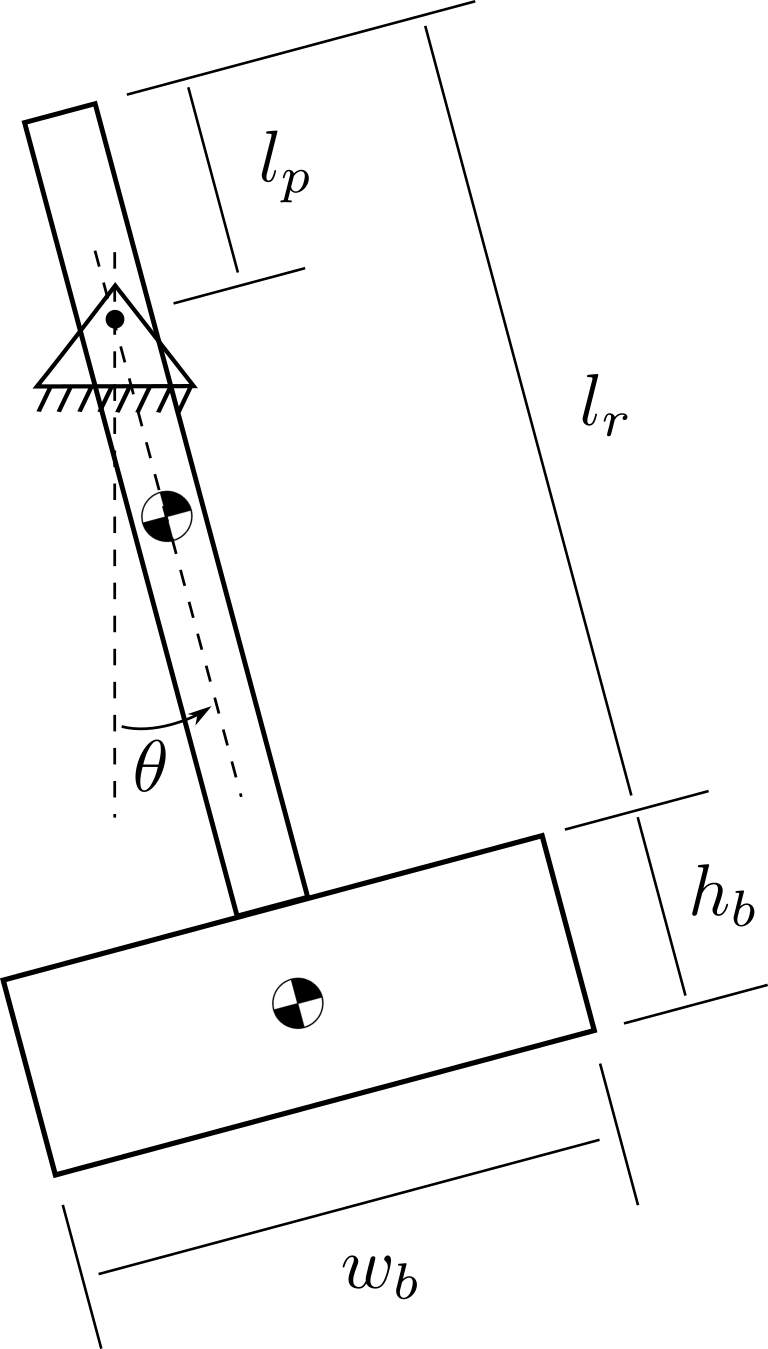
\includegraphics[scale=.125]{pendulum_fig1.png}

	\scalebox{1.0}{length of rod, $l_r=1.0$ (m)}\vspc
	\scalebox{1.0}{length to pivot, $l_p=0.25$ (m)}\vspc
	\scalebox{1.0}{height of block, $h_b=0.25$ (m)}\vspc
	\scalebox{1.0}{width of block, $w_b=0.5$ (m)}\vspc
	\scalebox{1.0}{mass of rod, $m_r=5$ (kg)}\vspc
	\scalebox{1.0}{mass of block, $m_b=25$ (kg)}\vspc		

\end{multicols}	        

\begin{framed}
\underline{Problem Statement} -  Derive the {\B equations of motion} using Newton's Second Law for the swinging pendulum shown.
\end{framed}

}


% Section II:
\section{\sectiontitleII}

\frame{
\frametitle{\sectiontitleII}

First, describe the model and list any important assumptions.
	\begin{itemize}
		\item The pendulum rigid and is composed a rod and a block. It rotates about the pin.\\
		\item Theta is positive in the counter-clockwise direction from the zero point (pointing down).\\
		\item There is no friction in the system. The pin joint is perfect and there is no air resistance. \\
		\item Gravity acts on the two center of gravity locations shown.\\
	\end{itemize}



}

% Section III:
\section{\sectiontitleIII}

% Section III - Frame I:
\frame{
\frametitle{\sectiontitleIII}

\textbf{ \Large \underline{Newton's Second Law Approach} }\\
\begin{enumerate}
\item Draw a {\BR Free Body Diagram}\vspc
\item Make an {\G assumption of motion}\vspc
\item Determine all {\B forces} acting on the system and their {\B directions}. \vspc
\item Write {\PR Newton's second law} for the appropriate DOF. \vspc\
\item Re-write the ODE in the {\PN standard form} of a system equation.
\end{enumerate}

}

% Section III - Frame II:
\frame{
\frametitle{\sectiontitleIII}

	Identify the forces acting on the rigid body. Because this a rotational problem we can ignore the reaction forces at the pin, but keep in mind the do exist and we could solve for them. Also, the radially forces will affect the moment, so they too can be ignored. We are left with the tangential forces. \vspc
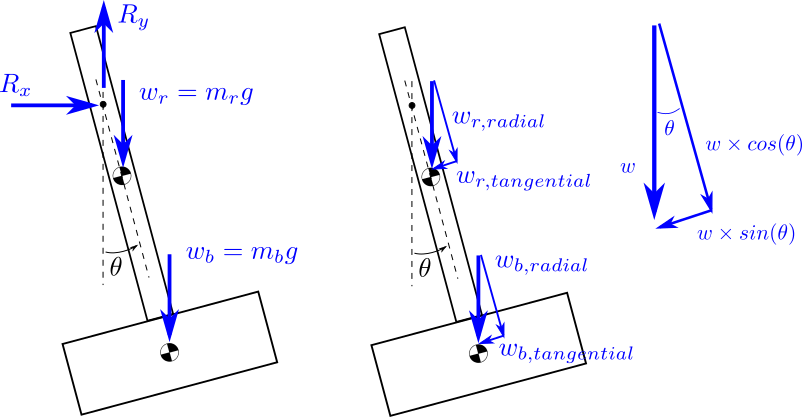
\includegraphics[scale=.35]{hw2_key_fig1.png} \vspc

}

% Section III - Frame III:
\frame{
\frametitle{\sectiontitleIII}

We need the perpendiculur moment arms from the forces to the pin. You have to be careful with the link lengths here. Define to new lengths $l_1$ as the lengths from the CG of the rod to pin and $l_2$ as the length from the CG of the block to the pin. \vspcc
$l_1=\frac{1}{2}l_r-l_p$ \vspc
$l_2=\frac{1}{2}l_r+\frac{1}{2}l_b+l_1$\vspc

}

% Section III - Frame III:
\frame{
\frametitle{\sectiontitleIII}
Now, determine the mass moment of inertia for the rigid body.\vspc
The intertia for the rod about the CG is define as:\vspc
$I_{r,CG}=\frac{1}{12}m_rl^2$\vspc
The intertia for the block about the CG is define as:\vspc
$I_{b,CG}=\frac{1}{12}m_b(h_b^2+w_b^2)$\vspc
They both must be translated to the pin joint using the {\it parallel axis theorem} so they can be summed.\vspc
$I_{r,o}=\frac{1}{12}m_rl^2+m_rl_1^2$\vspc
$I_{b,o}=\frac{1}{12}m_b(h_b^2+w_b^2)+m_bl_2^2$\vspc
$I_o=I_{r,o}+I_{b,o}=\frac{1}{12}m_rl^2+m_rl_1^2+\frac{1}{12}m_b(h_b^2+w_b^2)+m_bl_2^2$\vspc
}


% Section III - Frame IV:
\frame{
\frametitle{\sectiontitleIII}

Now we can write Newton's Second Law for rotation about a fixed point. The sum of the moments equals the mass moment of inertia times the angular acceleration.  \vspc
$\Sigma M_o=I_o\times\alpha=I_o\ddot{\theta}$ \vspc
$\Sigma M_o=-w_{r,tangential}\times l_1-w_{b,tangential}\times l_2=I_o\times\alpha=I_o\ddot{\theta}$ \vspc
$\Sigma M_o=-w_{r}\sin{\theta}\times l_1-w_{b}\sin{\theta}\times l_2=I_o\times\alpha=I_o\ddot{\theta}$ \vspc

Rearrange into the standard form of the {\it equation of motion}.  \vspc

$I_o\ddot{\theta}+(m_rgl_1+m_bgl_2)\sin{\theta}=0$ \vspc

}

% Section IV:
\section{\sectiontitleIV}

\frame{
\frametitle{\sectiontitleIV}

\begin{framed}
$I_o\ddot{\theta}+(m_rgl_1+m_bgl_2)\sin{\theta}=0$ \vspc
\end{framed}

with, \vspc
$l_1=(1/2)l_r-l_p$ \vspc
$l_2=(1/2)l_r+(1/2)l_b+l_1$ \vspc
and \vspc
$I_o=(1/12)m_rl^2+m_rl_1^2+(1/12)m_b(h_b^2+w_b^2)+m_bl_2^2$ \vspc



}
	
\end{document}





